\documentclass[tikz,border=4pt]{standalone}
\usepackage[T1]{fontenc}
\usepackage{newtxtext,newtxmath}
\usetikzlibrary{arrows.meta,positioning,calc}
\definecolor{ink}{HTML}{203B50}
\definecolor{bluefill}{HTML}{EFF4F8}
\definecolor{teal}{HTML}{236D71}
\definecolor{tealfill}{HTML}{EFF7F5}
\begin{document}
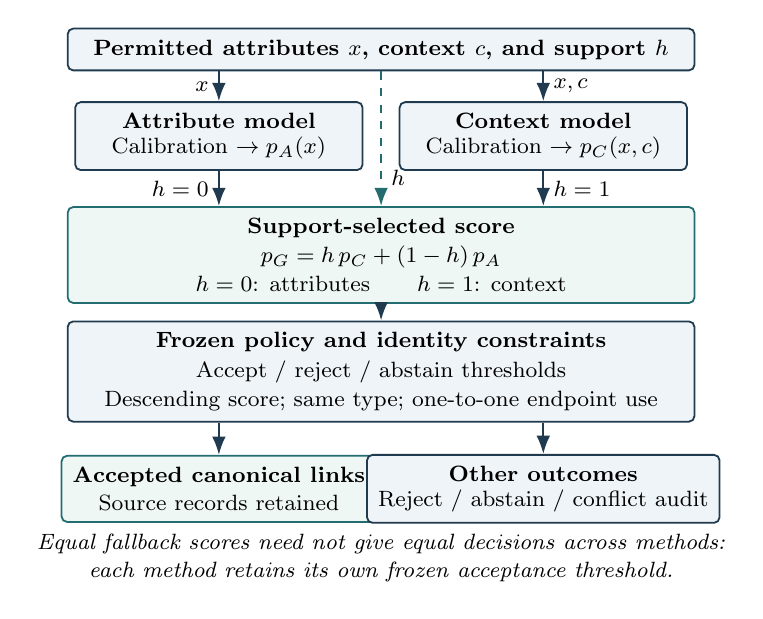
\begin{tikzpicture}[font=\fontsize{8.5}{10.7}\selectfont,>=Latex,
 box/.style={draw=ink,line width=.65pt,rounded corners=2pt,align=center,fill=bluefill,inner sep=4pt},
 flow/.style={->,draw=ink,line width=.8pt}]
\node[box,minimum width=7.96cm,minimum height=.50cm] (in) at (4.05,0) {\textbf{Permitted attributes $x$, context $c$, and support $h$}};
\node[box,minimum width=3.65cm,minimum height=.83cm] (a) at (1.99,-1.10) {\shortstack{\textbf{Attribute model}\\Calibration $\to p_A(x)$}};
\node[box,minimum width=3.65cm,minimum height=.83cm] (c) at (6.11,-1.10) {\shortstack{\textbf{Context model}\\Calibration $\to p_C(x,c)$}};
\draw[flow] (in.south -| a.north)--node[left,font=\fontsize{8}{9}\selectfont] {$x$} (a.north);
\draw[flow] (in.south -| c.north)--node[right,font=\fontsize{8}{9}\selectfont] {$x,c$} (c.north);
\node[box,draw=teal,fill=tealfill,minimum width=7.96cm,minimum height=1.03cm] (gate) at (4.05,-2.61) {\shortstack{\textbf{Support-selected score}\\$p_G=h\,p_C+(1-h)\,p_A$\\$h=0$: attributes\qquad $h=1$: context}};
\draw[flow,dashed,draw=teal] (in.south)--node[right,pos=.79,font=\fontsize{8}{9}\selectfont] {$h$} (gate.north);
\draw[flow] (a.south)--node[left,font=\fontsize{8}{9}\selectfont] {$h=0$} (a.south |- gate.north);
\draw[flow] (c.south)--node[right,font=\fontsize{8}{9}\selectfont] {$h=1$} (c.south |- gate.north);
\node[box,minimum width=7.96cm,minimum height=1.03cm] (policy) at (4.05,-4.09) {\shortstack{\textbf{Frozen policy and identity constraints}\\Accept / reject / abstain thresholds\\Descending score; same type; one-to-one endpoint use}};
\draw[flow] (gate.south)--(policy.north);
\node[box,draw=teal,fill=tealfill,minimum width=3.65cm,minimum height=.84cm] (ok) at (1.99,-5.58) {\shortstack{\textbf{Accepted canonical links}\\Source records retained}};
\node[box,minimum width=3.65cm,minimum height=.84cm] (audit) at (6.11,-5.58) {\shortstack{\textbf{Other outcomes}\\Reject / abstain / conflict audit}};
\draw[flow] (policy.south -| ok.north)--(ok.north);
\draw[flow] (policy.south -| audit.north)--(audit.north);
\node[align=center,font=\fontsize{7.8}{9.7}\selectfont\itshape] at (4.05,-6.46) {\shortstack{Equal fallback scores need not give equal decisions across methods:\\each method retains its own frozen acceptance threshold.}};
\end{tikzpicture}
\end{document}
